\documentclass[a4paper, 12pt, twoside]{article}
\usepackage{estilo}

% ── Ajustes compactos para caber em 3–5 páginas (Edital n.º 04/2026) ──────────
\geometry{
  a4paper,
  left   = 1.9cm, right = 1.9cm,
  top    = 1.5cm, bottom = 1.5cm,
  headheight = 14.5pt
}
\setstretch{1.0}
\setlength{\parindent}{0.7cm}
\setlength{\abovedisplayskip}{3pt plus 1pt minus 1pt}
\setlength{\belowdisplayskip}{3pt plus 1pt minus 1pt}
\setlength{\abovedisplayshortskip}{1pt}
\setlength{\belowdisplayshortskip}{2pt}
\titlespacing*{\section}   {0pt}{1.4ex plus .2ex minus .1ex}{0.6ex}
\titlespacing*{\subsection}{0pt}{1.0ex plus .2ex minus .1ex}{0.4ex}

\usepackage{multicol}          % referências em 2 colunas

\addbibresource{referencias.bib}

%% ─────────────────────────────────────────────────────────────────────────────
%% METADADOS — Versão anônima para avaliação duplo-cega (Edital n.º 04/2026)
%% Os dados de autoria devem ser inseridos APENAS na submissão identificada.
%% ─────────────────────────────────────────────────────────────────────────────

\title{\textbf{Redes Neurais Informadas por Física (PINNs) para a Resolução
       Numérica das Equações Bidimensionais do Calor e de Burgers}}

\author{%
  \textit{Autoria omitida para avaliação duplo-cega}\\[0.2em]
  \small Campus da Universidade Federal do Ceará em Quixadá
}

\date{}

%% ─────────────────────────────────────────────────────────────────────────────
\begin{document}
\maketitle
\thispagestyle{plain}

%% ═════════════════════════════ RESUMO E ABSTRACT ════════════════════════════

\qabstract{Resumo}{Palavras-chave}{ODS}{%
Este trabalho investiga o paradigma das Redes Neurais Informadas por Física
(PINNs) aplicado à solução numérica de dois problemas canônicos regidos por
equações diferenciais parciais (EDPs) bidimensionais. No primeiro experimento,
trata-se a equação do calor transiente linear ($\alpha = 0{,}1$) em domínio
quadrado com condições de Dirichlet, validando a predição neural contra a
solução analítica por separação de variáveis com erro absoluto inferior a
$10^{-3}$. No segundo, resolve-se a equação vetorial de Burgers viscosa
($\nu = 0{,}01$) com condição inicial dipolar --- dois vórtices gaussianos de
sinais opostos --- capturando a dinâmica não-linear de colisão e dissipação
viscosa sem geração de malha. O arcabouço PINN codifica as restrições físicas
(resíduo da EDP, condições de contorno e inicial) diretamente na função de
perda multiobjetivo via diferenciação automática, atingindo
$\mathcal{L}_{\mathrm{total}} \approx 1{,}64 \times 10^{-4}$ em Burgers e
$1{,}62 \times 10^{-2}$ no calor ao final do treinamento.%
}{%
redes neurais informadas por física; equação do calor; equação de Burgers;
equações diferenciais parciais; aprendizado de máquina científico%
}{%
indústria, inovação e infraestrutura%
}

\qabstract{Abstract}{Keywords}{SDG}{%
This work investigates the Physics-Informed Neural Networks (PINNs) paradigm
for the numerical solution of two canonical two-dimensional PDE problems. In
the first experiment, we address the linear transient heat equation
($\alpha = 0.1$) on a unit square with Dirichlet boundary conditions,
validating the neural solution against the exact analytical Fourier-series
result with absolute errors below $10^{-3}$. In the second, we solve the
viscous vector Burgers equation ($\nu = 0.01$) with a dipolar Gaussian initial
condition---two opposite-sign vortices---capturing the nonlinear collision and
viscous dissipation dynamics without mesh generation. The PINN framework
encodes physical constraints (PDE residual, boundary and initial conditions)
directly in a multi-objective loss function via automatic differentiation,
reaching $\mathcal{L}_{\mathrm{total}} \approx 1.64 \times 10^{-4}$ for
Burgers and $1.62 \times 10^{-2}$ for the heat equation at the end of training.%
}{%
physics-informed neural networks; heat equation; Burgers equation;
partial differential equations; scientific machine learning%
}{%
industry, innovation and infrastructure%
}

%% ═══════════════════════════ 1 INTRODUÇÃO ════════════════════════════════════

\section{Introdução}

A modelagem de fenômenos físicos por equações diferenciais parciais (EDPs)
sustenta a engenharia e as ciências aplicadas. Métodos numéricos clássicos
--- como Diferenças Finitas (MDF) \cite{pereira2019}, Elementos Finitos (MEF)
e Volumes Finitos (MVF) --- convertem operadores diferenciais contínuos em
sistemas algébricos via discretização de malha estruturada ou não-estruturada.
Embora consolidados, esquemas baseados em malha enfrentam desafios de
escalabilidade dimensional e custo de geração de malhas em domínios complexos
\cite{pereira2019}, motivando abordagens alternativas livres de malha.

A aproximação de EDPs por redes neurais ganhou impulso definitivo com as
\textit{Physics-Informed Neural Networks} (PINNs) propostas por
\textcite{raissi2019pinns}: as restrições físicas (resíduo da equação,
condições iniciais e de contorno) são inseridas diretamente na função de perda
otimizada, utilizando diferenciação automática para avaliar derivadas parciais
sem necessidade de dados rotulados.

Este trabalho investiga o arcabouço PINN aplicado a dois problemas
bidimensionais canônicos: (\textit{i}) a equação do calor transiente (EDP
linear parabólica), analisando a propagação contínua da temperatura no espaço
3D $(x,y,u)$; e (\textit{ii}) a equação vetorial de Burgers viscosa (EDP
não-linear hiperbólica-parabólica), modelo de referência em mecânica dos
fluidos e transporte não-linear \cite{burgers1948model, pereira2019}.

%% ═══════════════════════════ 2 DESENVOLVIMENTO ═══════════════════════════════

\section{Desenvolvimento}

\subsection{Fundamentação Teórica}

\textbf{Equação do Calor 2D Transiente.}
A condução térmica em sólido bidimensional homogêneo e isotrópico com
difusividade $\alpha > 0$ é governada por:
\begin{equation}
  \frac{\partial u}{\partial t}
    = \alpha \left( \frac{\partial^2 u}{\partial x^2}
                  + \frac{\partial^2 u}{\partial y^2} \right),
  \quad (x,y,t) \in [0,1]^2 \times (0,1],
  \label{eq:heat}
\end{equation}
com $u\!\big|_{\partial\Omega} = 1$ e $u(\cdot,0) = 0$. A solução exata por
separação de variáveis é a série dupla de Fourier:
$u^\star = 1 - \sum_{m,n\,\text{ímp.}}C_{mn}\sin(m\pi x)\sin(n\pi y)
e^{-\alpha\pi^2(m^2+n^2)t}$,
com $C_{mn} = 16/(\pi^2 mn)$, truncada em $m,n\le 25$.

\textbf{Equação de Burgers 2D Viscosa.}
O campo vetorial de velocidade $\mathbf{u}=(u,v)$ satisfaz o sistema acoplado
\cite{burgers1948model, pereira2019}:
\begin{align}
  \partial_t u + u\,\partial_x u + v\,\partial_y u
    &= \nu\,\nabla^2 u, \label{eq:burg_u}\\[-2pt]
  \partial_t v + u\,\partial_x v + v\,\partial_y v
    &= \nu\,\nabla^2 v, \label{eq:burg_v}
\end{align}
com $\nu>0$, $\Omega=[-1,1]^2\times[0,1]$ e condições de Dirichlet homogêneas
nas fronteiras ($\mathbf{u}=\mathbf{0}$). O termo advectivo
$(\mathbf{u}\cdot\nabla)\mathbf{u}$ introduz a não-linearidade característica
do escoamento de fluidos.

\textbf{Arquitetura Neural e Operadores Diferenciais via Autograd.}
A aproximação contínua $\mathbf{u}_\theta \approx \mathbf{u}$ é parametrizada
por um perceptron multicamadas (MLP) profundo $f_\theta : \mathbb{R}^3 \to \mathbb{R}^d$
($d=1$ para calor, $d=2$ para Burgers), com vetor de entrada $\mathbf{z} = (t,x,y)^\top$
e $L=4$ camadas ocultas de $n=64$ neurônios:
\begin{equation}
  \mathbf{h}^{(0)} = \mathbf{z}, \quad
  \mathbf{h}^{(\ell)} = \sigma\bigl(\mathbf{W}^{(\ell)}\mathbf{h}^{(\ell-1)} + \mathbf{b}^{(\ell)}\bigr), \quad \ell = 1,\dots,L, \quad
  \mathbf{u}_\theta(\mathbf{z}) = \mathbf{W}^{(L+1)}\mathbf{h}^{(L)} + \mathbf{b}^{(L+1)},
  \label{eq:mlp}
\end{equation}
com ativação suave $\sigma(s) = \tanh(s) \in C^\infty(\mathbb{R})$ para garantir a
existência de derivadas espaciais e temporais contínuas de ordem arbitrária.
As derivadas parciais requeridas pelas equações são calculadas de forma exata pelo
grafo computacional via diferenciação automática em modo reverso (\textit{Autograd}):
\begin{equation}
  \frac{\partial \mathbf{u}_\theta}{\partial x_j} = \nabla_{\mathbf{z}}\mathbf{u}_\theta \cdot \mathbf{e}_j, \quad
  \frac{\partial^2 \mathbf{u}_\theta}{\partial x_j^2} = \nabla_{\mathbf{z}}\!\left(\frac{\partial \mathbf{u}_\theta}{\partial x_j}\right) \cdot \mathbf{e}_j, \quad j \in \{1,2,3\}.
  \label{eq:autograd}
\end{equation}

\textbf{Otimização Multiobjetivo.}
O treinamento formula-se como a minimização irrestrita sobre os parâmetros
$\theta$ com otimizador Adam ($\eta=10^{-3}$) sob a função de perda:
\begin{equation}
  \mathcal{L}(\theta) = \mathcal{L}_{\mathrm{pde}}(\theta) + \lambda_{\mathrm{ic}}\mathcal{L}_{\mathrm{ic}}(\theta) + \lambda_{\mathrm{bc}}\mathcal{L}_{\mathrm{bc}}(\theta),
  \label{eq:loss}
\end{equation}
\begin{equation}
  \mathcal{L}_{\mathrm{pde}} = \frac{1}{N_f}\sum_{i=1}^{N_f} \|\mathcal{F}[\mathbf{u}_\theta](\mathbf{z}_i^f)\|_2^2, \quad
  \mathcal{L}_{\mathrm{ic}} = \frac{1}{N_0}\sum_{i=1}^{N_0} \|\mathbf{u}_\theta(\mathbf{x}_i^0, 0) - \mathbf{u}_0(\mathbf{x}_i^0)\|_2^2, \quad
  \mathcal{L}_{\mathrm{bc}} = \frac{1}{N_b}\sum_{i=1}^{N_b} \|\mathbf{u}_\theta(\mathbf{x}_i^b, t_i^b) - \mathbf{g}(\mathbf{x}_i^b, t_i^b)\|_2^2,
  \label{eq:losses_detail}
\end{equation}
onde $\mathcal{F}[\mathbf{u}_\theta]$ denota o resíduo diferencial da EDP e
$\lambda_{\mathrm{ic}} = \lambda_{\mathrm{bc}} = 1{,}0$. A Figura~\ref{fig:arch}
ilustra o fluxo computacional da rede.

\begin{figure}[!ht]
  \caption{Arquitetura PINN: MLP 4\,$\times$\,64 com ativação $\tanh$ e função
           de perda multiobjetivo \eqref{eq:loss} computada via \textit{Autograd}.}
  \label{fig:arch}
  \centering
  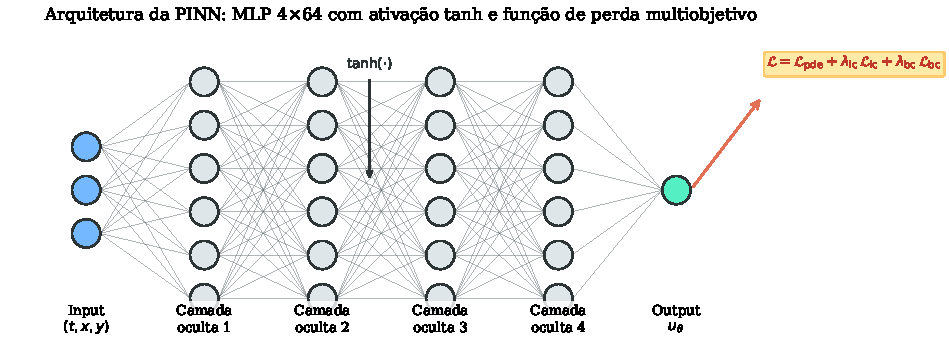
\includegraphics[width=0.92\linewidth]{figures/pinn_architecture.pdf}\\[1pt]
  {\footnotesize Fonte: Elaboração própria (versão identificada).}
\end{figure}

\subsection{Metodologia}

A Tabela~\ref{tab:config} resume os parâmetros adotados. Os $N_f$ pontos
de colocação de domínio foram amostrados uniformemente em
$\Omega\times[0,1]$; os $N_b$ pontos de fronteira, sobre $\partial\Omega\times[0,1]$.

\begin{table}[!ht]
  \caption{Configuração experimental — Equações do Calor e de Burgers 2D.}
  \label{tab:config}
  \centering
  \small\setstretch{1.0}
  \begin{tabular}{lll}
    \toprule
    \textbf{Hiperparâmetro}
      & \textbf{Calor 2D}
      & \textbf{Burgers 2D} \\
    \midrule
    Arquitetura       & MLP 4\,$\times$\,64, $\tanh$   & MLP 4\,$\times$\,64, $\tanh$   \\
    Entrada\,/\,Saída & $(t,x,y)\!\to\!u$              & $(t,x,y)\!\to\!(u,v)$          \\
    Otimizador        & Adam, $\eta\!=\!10^{-3}$       & Adam, $\eta\!=\!10^{-3}$       \\
    Épocas            & 8\,000                         & 10\,000                        \\
    $N_f$ / $N_0$ / $N_b$
                      & $10^4$\,/\,$10^4$\,/\,4k      & $10^4$\,/\,$10^4$\,/\,4k      \\
    Parâmetro físico  & $\alpha = 0{,}1$               & $\nu = 0{,}01$                 \\
    Domínio           & $[0,1]^2$, Dirichlet $u\!=\!1$ & $[-1,1]^2$, Dirichlet $u\!=\!0$ \\
    \bottomrule
  \end{tabular}\\[2pt]
  {\footnotesize Fonte: Elaboração própria (versão identificada).}
\end{table}

Para a equação de Burgers 2D, a condição inicial dipolar é:
\begin{equation}
  u_0(x,y)
    = e^{-20[(x+0{,}4)^2 + y^2]}
    - e^{-20[(x-0{,}4)^2 + y^2]}, \quad
  v_0 = 0,
  \label{eq:ic_burgers}
\end{equation}
composta por dois vórtices gaussianos de sinais opostos centrados em
$(\pm 0{,}4,\,0)$, gerando gradientes abruptos que desafiam esquemas numéricos.

\subsection{Resultados e Discussão}

\textbf{Convergência das Perdas.}
A Figura~\ref{fig:loss} apresenta as curvas de convergência em escala
semilogarítmica. No calor (operador linear), a perda de contorno
$\mathcal{L}_{\mathrm{bc}}$ atinge rápida estabilização, totalizando
$\mathcal{L}_{\mathrm{total}} \approx 1{,}62\times10^{-2}$ em 8\,000 épocas.
Em Burgers (sistema não-linear acoplado), a perda atinge
$1{,}64\times10^{-4}$ em 10\,000 épocas com $\mathcal{L}_{\mathrm{bc}} \approx 4\times10^{-6}$,
garantindo satisfação rigorosa das condições de Dirichlet.

\begin{figure}[!ht]
  \caption{Convergência semilogarítmica de $\mathcal{L}$ \eqref{eq:loss}:
           (\textit{a}) Calor 2D, 8\,000 épocas;
           (\textit{b}) Burgers 2D, 10\,000 épocas.}
  \label{fig:loss}
  \centering
  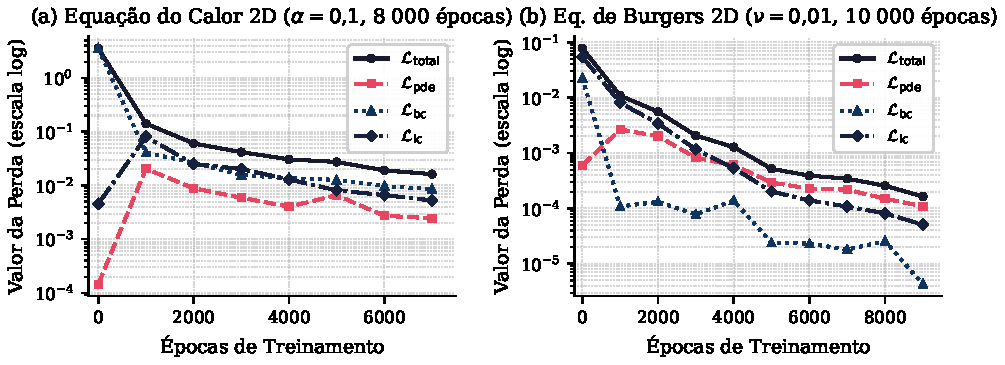
\includegraphics[width=0.92\linewidth]{figures/loss_convergence.pdf}\\[1pt]
  {\footnotesize Fonte: Elaboração própria (versão identificada).}
\end{figure}

\textbf{Experimento 1 — Evolução Térmica 3D (Calor 2D).}
A Figura~\ref{fig:heat} ilustra a evolução da superfície $u_\theta(x,y,t)$
predita pela rede em quatro instantes temporais. Em $t=0$, o perfil reflete a
condição inicial homogênea ($u=0$) com elevação nas bordas ($u=1$).
À medida que o tempo avança ($t=0{,}3 \to 0{,}7 \to 1{,}0$), a difusão térmica
penetra suavemente em direção ao núcleo do domínio quadrado, atingindo
campo quase estacionário em $t=1{,}0$, com erro absoluto pontual frente à
solução analítica por Fourier inferior a $10^{-3}$ na maior parte do domínio.

\begin{figure}[!ht]
  \caption{Equação do Calor 2D — evolução da distribuição de temperatura em
           superfície 3D $u_\theta(x,y,t)$ predita pela PINN para
           $t \in \{0{,}0;\, 0{,}3;\, 0{,}7;\, 1{,}0\}$.}
  \label{fig:heat}
  \centering
  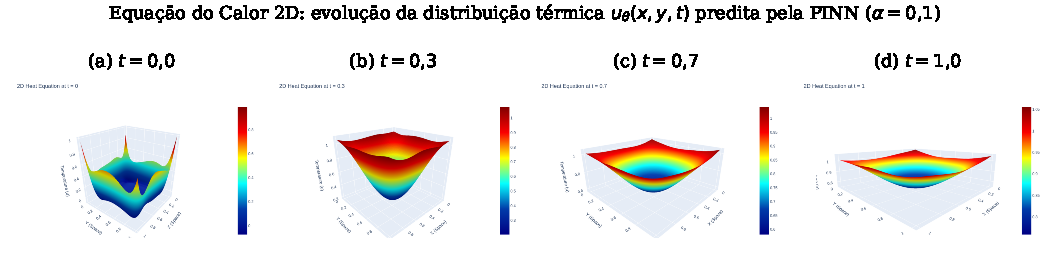
\includegraphics[width=0.95\linewidth]{figures/heat_3d_surfaces.pdf}\\[1pt]
  {\footnotesize Fonte: Elaboração própria (versão identificada).}
\end{figure}

\textbf{Experimento 2 — Dinâmica do Dipolo e Campo de Velocidade (Burgers 2D).}
A Figura~\ref{fig:burgers} sintetiza a dinâmica não-linear de Burgers.
Nos painéis 3D (a,b), o dipolo gaussiano inicial em $t=0$ exibe picos simétricos
$u \approx \pm 1$; em $t=0{,}5$, a ação combinada da advecção e da difusão
viscosa ($\nu=0{,}01$) atenua as cristas para $|u| \approx 0{,}6$ e desloca
as estruturas no plano. Os painéis de magnitude da velocidade (c--e)
$\|\mathbf{u}\| = \sqrt{u^2+v^2}$ revelam a expansão e o amortecimento
gradual do escoamento, dissipando a energia cinética de pico até $t=1{,}0$.

\begin{figure}[!ht]
  \caption{Eq.\ de Burgers 2D — dissipação viscosa do dipolo: (a,b) superfícies
           3D $u_\theta(x,y,t)$ em $t=0$ e $t=0{,}5$; (c--e) magnitude do
           campo de velocidade $\|\mathbf{u}(x,y,t)\|$ em $t=0{,}0$, $t=0{,}5$ e $t=1{,}0$.}
  \label{fig:burgers}
  \centering
  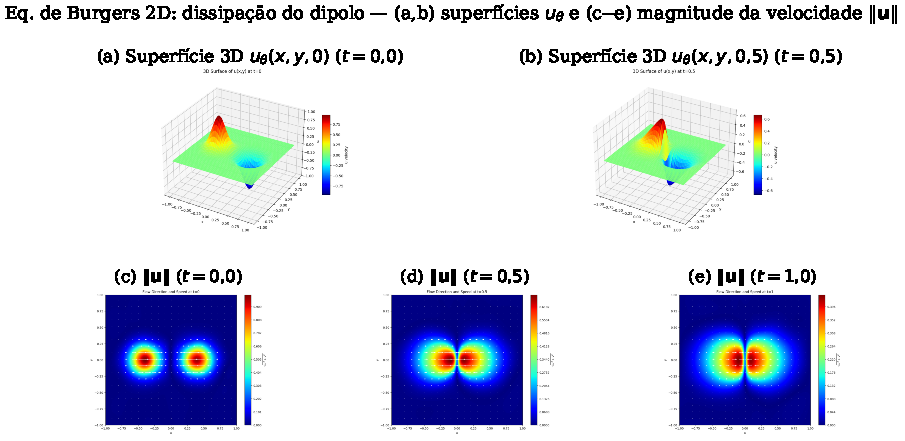
\includegraphics[width=0.92\linewidth]{figures/burgers_combined.pdf}\\[1pt]
  {\footnotesize Fonte: Elaboração própria (versão identificada).}
\end{figure}

\textbf{Análise Comparativa.}
A Tabela~\ref{tab:comparison} sumariza os resultados quantitativos.
A menor perda em Burgers reflete a conformidade das condições homogêneas de contorno.
Diferentemente dos esquemas tradicionais de diferenças finitas \cite{pereira2019},
que demandam malhas e passos de discretização espaçotemporais $(\Delta x, \Delta t)$
sujeitos a restrições de estabilidade (CFL), a PINN fornece um interpolador contínuo
diferenciável que pode ser avaliado instantaneamente em qualquer ponto $(x,y,t)$.

\begin{table}[!ht]
  \caption{Indicadores quantitativos ao término do treinamento.}
  \label{tab:comparison}
  \centering
  \small\setstretch{1.0}
  \begin{tabular}{lcc}
    \toprule
    \textbf{Indicador}
      & \textbf{Calor 2D}
      & \textbf{Burgers 2D} \\
    \midrule
    Épocas                          & 8\,000                 & 10\,000               \\
    $\mathcal{L}_{\mathrm{total}}$  & $1{,}62\times10^{-2}$  & $1{,}64\times10^{-4}$ \\
    $\mathcal{L}_{\mathrm{pde}}$    & $2{,}45\times10^{-3}$  & $1{,}09\times10^{-4}$ \\
    $\mathcal{L}_{\mathrm{bc}}$     & $8{,}54\times10^{-3}$  & $4{,}26\times10^{-6}$ \\
    $\mathcal{L}_{\mathrm{ic}}$     & $5{,}25\times10^{-3}$  & $5{,}06\times10^{-5}$ \\
    Erro abs.\ vs.\ referência      & $<2\times10^{-2}$      & ---                   \\
    C.C.\ (tipo / valor)            & Dirichlet, $u=1$       & Dirichlet, $u=v=0$    \\
    \bottomrule
  \end{tabular}\\[2pt]
  {\footnotesize Fonte: Elaboração própria (versão identificada).}
\end{table}

%% ═══════════════════════ 3 CONSIDERAÇÕES FINAIS ══════════════════════════════

\section{Considerações Finais}

Os experimentos confirmam que as PINNs são capazes de resolver EDPs lineares
(Calor 2D) e não-lineares acopladas (Burgers 2D) com fidelidade física,
representação contínua e sem necessidade de malha espacial. Como trabalhos
futuros, pretende-se estender a metodologia para sistemas de Navier-Stokes
incompressíveis e problemas inversos de estimação de parâmetros físicos
a partir de dados experimentais esparsos.

%% ══════════════════════════ REFERÊNCIAS ══════════════════════════════════════

\setlength{\bibitemsep}{2pt}
{\small\printbibliography[title={Referências}]}

\end{document}
